\documentclass{99-Styles/MICE}
\usepackage{bm} % For formatting math mode in bold
\usepackage{amsmath}
\usepackage{graphicx}

%
\input 99-Styles/GetPackages

\linenumbers
\modulolinenumbers[5]
\begin{document}

\input 00a-Top-matter/00a-Top-matter

%\makeatletter

\input 99-Styles/MICE-defs

\parindent 10pt
\pagestyle{plain}
\pagenumbering{arabic}                   
\setcounter{page}{1}

\input 00b-Abstract/00b-Abstract
\section{The MICE Experiment}
\label{sec:MICE}
  \subsection{Overview}
  \label{subsec:Overview}
  The Muon Ionization Cooling Experiment (MICE) will perform a practical demonstration of muon ionization cooling. Cooling refers to a reduction in the emittance of a beam, that is, the reduction of the phase-space volume occupied by the beam. Beam cooling is required for any future facility based on high intensity muon beams, such as a Neutrino Factory~\cite{ISS-Physics}, the ultimate tool to study leptonic CP-invariance violation, or a Muon Collider~\cite{MC_Overview}, a potential route to multi-TeV lepton -- anti-lepton collisions. Muon beams are generated via pion decay, and therefore have a large emittance, which must be reduced so that a reasonable fraction of the beam will fall within the acceptance of the downstream acceleration system.

  The short muon lifetime requires fast beam cooling that traditional techniques are unable to provide.  Ionization cooling was proposed in the early 1970s~\cite{Skrinsky, Neuffer}, but has not yet been demonstrated at the energies of interest for the Neutrino Factory or Muon Collider.  Ionization cooling reduces emittance by passing a beam through some suitable material of low atomic-number such as liquid hydrogen.  This leads to the reduction of all components of momentum due to ionization energy loss. Low atomic number absorbers are preferred because they minimise multiple scattering which ``heats'' the beam. %After the absorber, momentum is restored in the longitudinal direction only by means of radio frequency cavities.  The sequence is repeated leading to an overall reduction in the transverse phase-space occupied by the beam.

  \begin{figure}[bht]
    \begin{center}
      \includegraphics[width=1.0\linewidth]{01-MICE/Cooling-demo-labels.pdf}
      \caption{\label{fig:CoolingChannel} The beam diagnostics and cooling cell (indicated in green). $M$ refers to matching coils, $E$ to end coils and $C$ to the centre coils. Particle identification is provided by three time-of-flight stations, two threshold Cherenkov detectors and a downstream calorimeter composed of a pre-shower detector and an electron-muon ranger. Emittance is measured upstream and downstream of the cooling cell using spectrometers. A diffuser is used to increase the beam emittance prior to the upstream spectrometer. Ionization energy loss occurs as the beam passes through the absorbers, while acceleration is providing by radio frequency cavities.}
    \end{center}
  \end{figure}

  MICE is sited at the Science and Technology Facilities Council Rutherford Appleton Laboratory in the U.K. and exploits the ISIS proton synchrotron to generate the muon beam~\cite{MiceTarget}.  The MICE beam line is described in detail in~\cite{BeamlineJINST}. A schematic of the full MICE experiment is shown in figure~\ref{fig:CoolingChannel}. The beamline is instrumented with with two threshold Cherenkov detectors, three time-of-flight (TOF) stations and a downstream calorimeter. The cooling cell consists of three absorber modules and two radio frequency (RF) cavities. Two high-precision trackers in a solenoidal field are used to measure the emittance change (see section~\ref{subsec:Trackers}).

  MICE is a staged experiment, built and run in distinct steps. The first step of the programme, consisting of the muon beam line with particle identification, is now complete and results are available in~\cite{BeamlineJINST, BeamCharacterisationEurPhysJ, EMRJINST, PionContaminationJINST}. The present step of the program, which introduced the trackers and the first absorber module, began taking data in 2015. % The demonstration of sustainable cooling, which includes longitudinal re-acceleration, will begin data taking in 2018.

%   \begin{figure}[tb]
%     \begin{center}
%       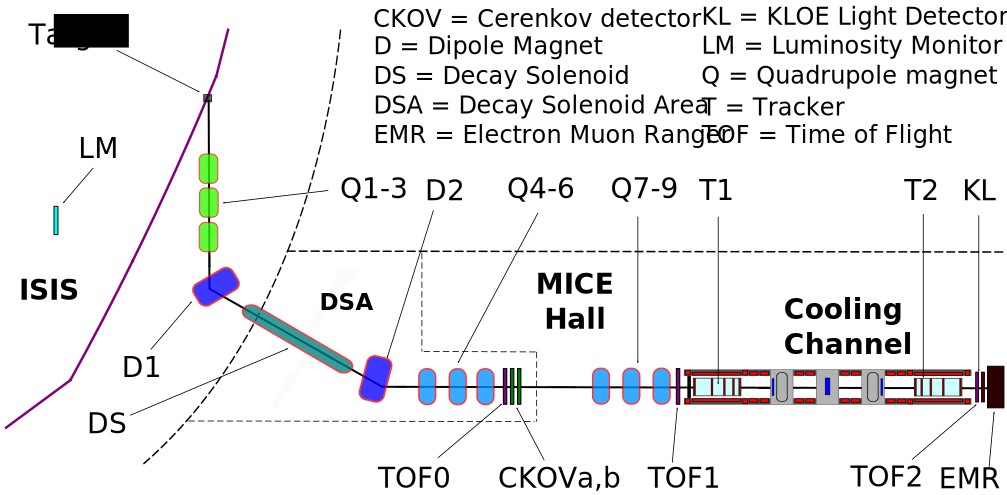
\includegraphics[width=0.75\linewidth]{01-MICE/BeamLineDEMOSans.pdf}
%       \caption{\label{fig:Beamline}The MICE Muon Beamline. A pion production target intercepts the protons of the circulating ISIS beam. Some of the subsequent pions are then captured by quadrupoles and guided down the beam line, passing through various PID detectors along the way, before delivery to the cooling cell itself. Emittance is measured immediately before and after the cooling cell using the scintillating-fibre trackers.}
%       \end{center}
%   \end{figure}

  \subsection{The Scintillating Fibre Trackers}
  \label{subsec:Trackers}
  MICE is equipped with two identical, high precision scintillating-fibre (``scifi'') trackers, described in~\cite{TrackersNIM}. Each tracker is placed in a superconducting solenoid that provides a uniform field over the tracking volume. One tracker, TKU, is upstream of the cooling cell, the other, TKD, downstream.  Each tracker consists of 5 detector stations, labelled 1 to 5, as illustrated in figure~\ref{fig:Trackers}. TKU is orientated such that Station~5 sees the beam first, TKD is rotated by 180$^\circ$ such that Station~1 sees the beam first, thus, in both trackers, Station~1 is always nearest to the cooling cell (see figure~\ref{fig:CoolingChannel}).
 

  Each station is formed of three planes of 350~$\mu$m scintillating-fibres, orientated at 120 degrees to one another. The fibres in each plane are arranged in two layers offset with respect to each other (a ``doublet layer''), in order to give 100$\%$ coverage of the plane area as illustrated in figure~\ref{fig:DoubletLayer}. The doublet layer is glued on to a sheet of mylar. The fibres are collected into groups of seven for readout, each group forming a single channel, as illustrated in figure~\ref{fig:DoubletLayer}b. The planes, also known as views, are labelled $U$, $V$ and $W$. Plane $U$ is attached to the station frame directly, plane $W$ on to plane $U$, and plane $V$ on to plane $W$. The fibre-plane orientations are illustrated in figure~\ref{fig:FibrePlaneOrientation}. Each station is oriented such that the fibres in the $U$ plane are vertical. The fibres produce scintillation light when ionizing radiation passes through them. Clear-fibre light guides transport the scintillation light to visible light photon counters (VLPCs) that are operated at 9~$K$ in a cryostat~\cite{TrackersNIM}. The signal from the VLPCs is digitised using front-end electronics developed by the D0 experiment~\cite{D0}. %See~\cite{TrackersNIM} for details.
  
  \begin{figure}[tb]
    \centering
    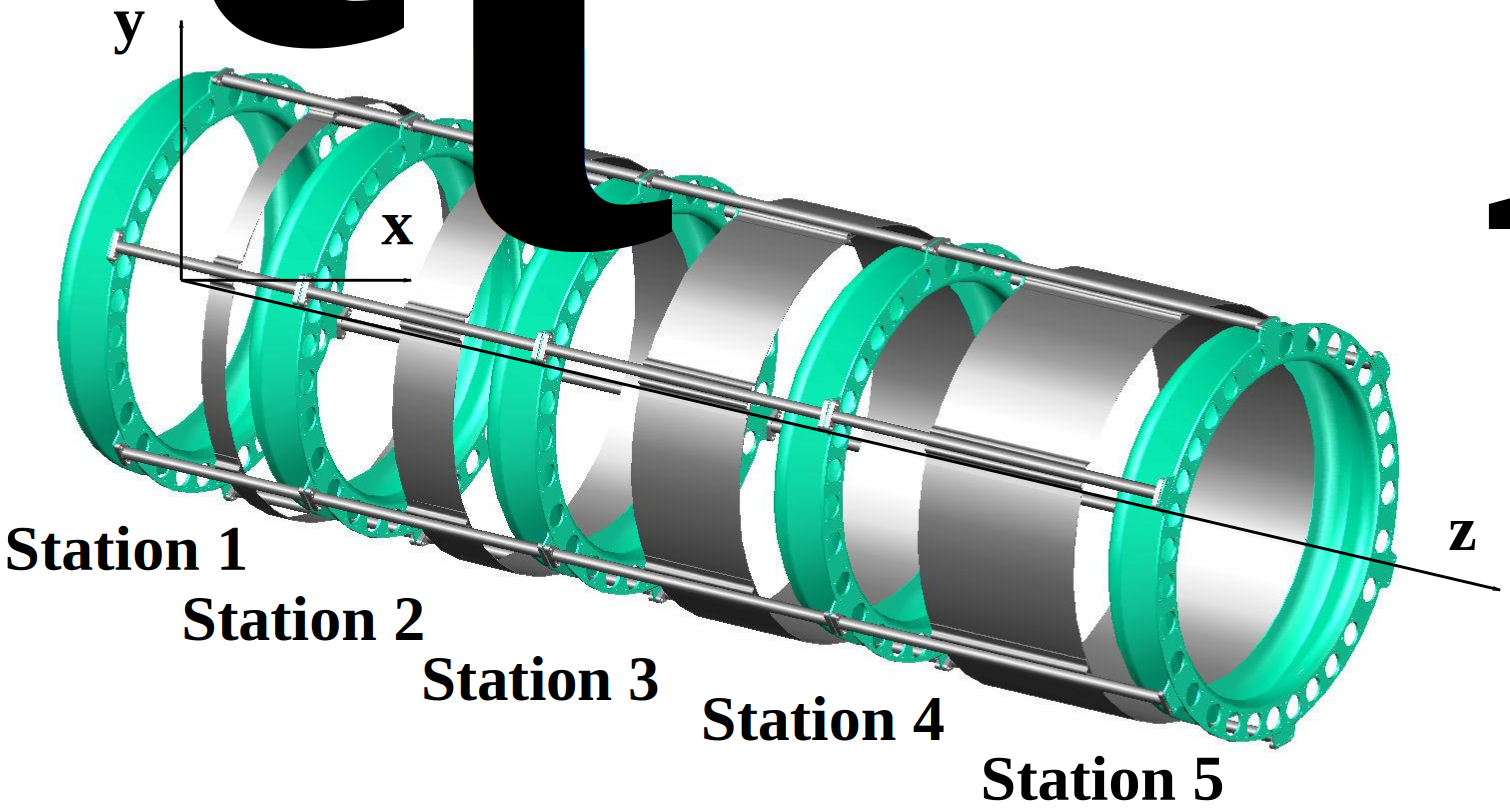
\includegraphics[width=0.5\linewidth]{01-MICE/TrackerFrame.pdf} \hspace{2pc}%
    \includegraphics[width=0.35\linewidth]{01-MICE/TrackerPhoto.pdf}
    \caption{\label{fig:Trackers} Left: A schematic of the tracker carbon-fibre frame.  The fibre planes are glued on to the upstream edge of the carbon-fibre station frames (shown in green). The longitudinal coordinate of the tracker coordinate system ($z_t$) increases as one moves from the fibre plane towards the station frame to which it is attached.  Right: A photograph of a tracker. The colour is due to the filtered lighting needed to protect the scintillating-fibres. The intersecting lines visible on the station faces indicate the direction of the fibres in each plane.}
  \end{figure}

  \begin{figure}[tb]
    \begin{center}
      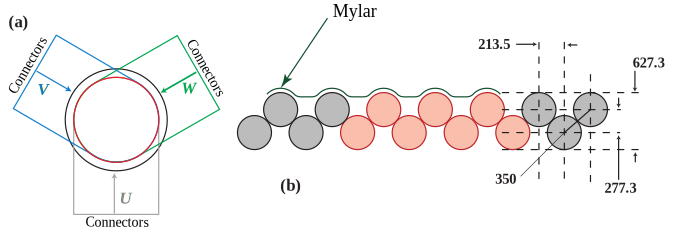
\includegraphics[width=0.85\textwidth]{01-MICE/doublet-layer.pdf}
      \caption{\label{fig:DoubletLayer}(a) Arrangement of the doublet layers in the scintillating-fibre  stations. The outer circle shows the solenoid bore while the inner circle shows the limit of the active area of the tracker. The arrows indicate the direction that the individual 350\,$\mu$m fibres run. (b) Detail of the arrangement of the scintillating-fibres in a doublet layer. The fibre spacing and the fibre pitch are indicated on the right-hand end of the figure in \,$\mu$m. The pattern of seven fibres shown in red form a single channel, which is readout via a clear-fibre light-guide. The sheet of mylar glued to the doublet layer is indicated. }
    \end{center}
  \end{figure}

  \begin{figure}[tb]
    \centering
    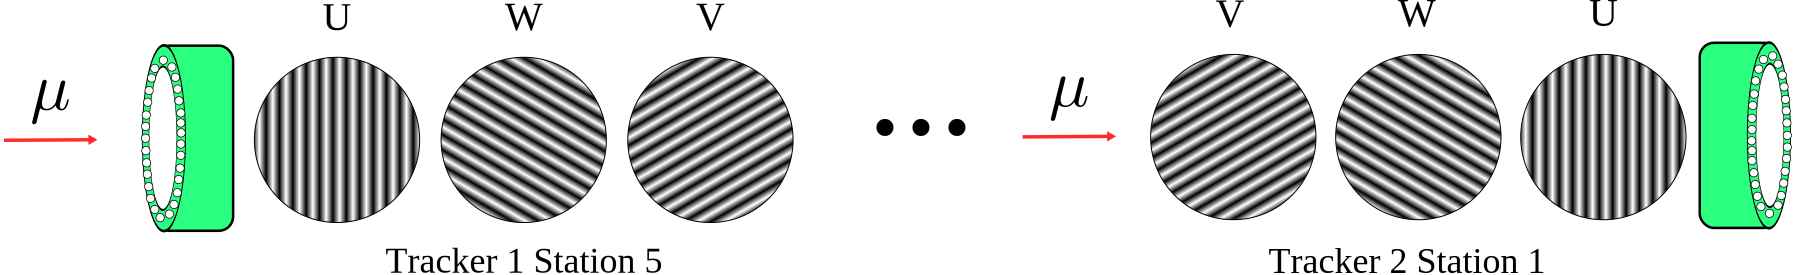
\includegraphics[width=0.95\linewidth]{01-MICE/FibrePlaneOrientation.pdf} \hspace{2pc}%
    \caption{\label{fig:FibrePlaneOrientation} The orientation of the fibres in each plane, as seen by the incoming beam, for both trackers. The green object is the station frame.}
  \end{figure}
\section{Coordinate systems and Reference Surfaces}
\label{sec:Coordinates}

  \subsection{Channels and Digits}
  The $V$ and $W$ planes each consist of 214 channels, labelled 0 to 213, while the $U$ plane has 212 channels, labelled 0 to 211.  The channel number increases from left to right if a plane is placed mylar side up, with the fibre readout pointing downwards, as illustrated in figure~\ref{fig:DoubletLayerOrder}.

  \subsection{Planes and Clusters}
  \label{subsec:PlaneAndClusters}
  The plane reference surface is defined to be the flat plane that is formed by the outer surface of the mylar sheet. The measured position perpendicular to the direction of the fibres in each plane is labelled  $\alpha \in (v, u, w)$, defined to increase in the \textit{opposite} direction to the channel number. $\alpha$ is then given by:
  
  \begin{equation}
   \alpha = \left(N_{CC} - N_{Ch}\right) \times p \times d
  \end{equation}

  \noindent
  where $N_{CC}$ is the central channel number, $N_{Ch}$ is the channel number, $p$ is the channel pitch, that is twice the horizontal distance between neighbouring fibres ($2 \times 213.5 = 417$~mm) , and $d$ is half the number of fibres in a channel, i.e. $3.5$ (see figure~\ref{fig:DoubletLayer}, it can be seen $p \times d$ is just the width of a channel).  
  
  The $z$ axis of the plane coordinate system is defined to be perpendicular to the plane reference surface and points in the direction from the mylar sheet towards the fibres. The direction in which the fibres run defines the final plane coordinate, $\beta$, with the direction defined to complete a right-handed coordinate system. The origin of the $(\alpha, \beta)$ coordinate system is taken to be at the centre of the circular active area of the plane.

  \subsection{Stations and Spacepoints}
  The station reference surface is defined to coincide with the reference surface of the $V$ doublet-layer. The station coordinate system is defined such that the $x_s$ axis is coincident with the $V$ layer, the $z_s$ axis is coincident with the $z_p$ axis of the $V$ layer and the $y_s$ axis completes a right-handed coordinate system.

  \subsection{Trackers and Tracks}
  The tracker reference surface is defined to coincide with the reference surface of Station~1. The tracker coordinate system is defined such that the $z_t$ axis coincides with the axis of cylindrical symmetry of the tracker as shown in figure~\ref{fig:Trackers}. The tracker $z_t$ coordinate increases from Station~1 to Station~5. The tracker $y_t$ axis is defined to coincide with the $y_s$ axis of Station~1 and the tracker $x_t$ axis completes a right-handed coordinate system. 
  
  \begin{figure}[htb]
    \begin{center}
      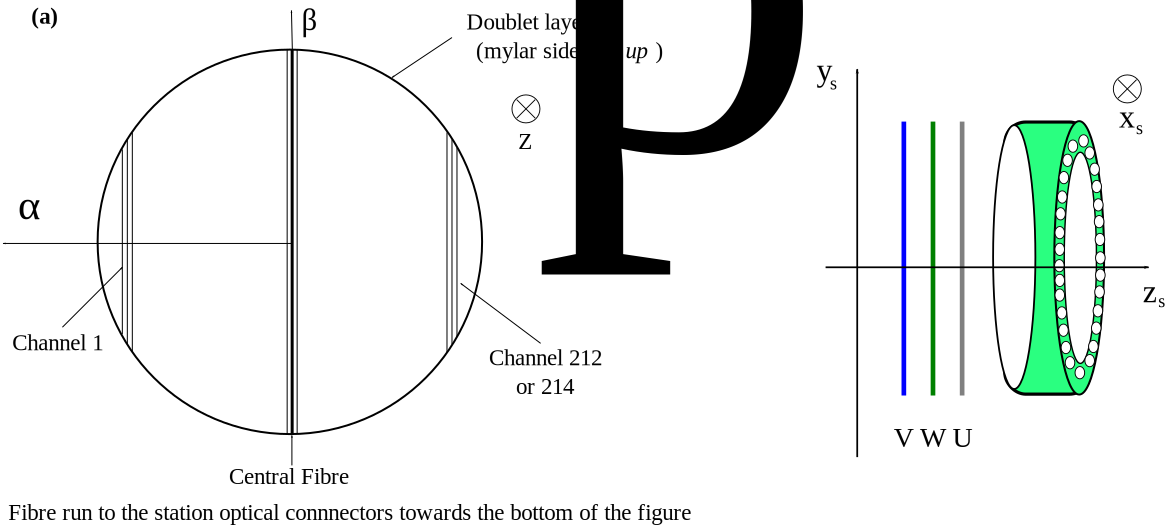
\includegraphics[width=0.9\textwidth]{02-CoordinateSystems/PlaneCoordinatesAndNumbering.pdf}
      \caption{\label{fig:DoubletLayerOrder} (a)~The channel numbering within a plane, and the $(\alpha, \beta, z_p)$ plane coordinate system (a right-handed system).  (b)~The fibre plane ordering with respect to the station body and the station coordinate frame (a right-handed system).  In TKU the beam approaches from the right, in TKD from the left. Note that $z_s$ is by definition equivalent to $z_p$ of the $V$ plane.}
    \end{center}
  \end{figure}


\section{The MAUS Framework}
\label{sec:MAUS}
The tracker software is part of the MICE software framework, known as MAUS (MICE Analysis User Software)~\cite{MausPaper}. MAUS is used to perform Monte Carlo simulation and both online and offline data reconstruction. It is built using a combination of C++ and Python, with C++ being used predominantely in the code used for more processor intensive tasks (the ``backend'') and Python being used more in the code presented to the user (the``frontend'').  Simulation is supported by GEANT4~\cite{GEANT4}, and analysis with ROOT~\cite{ROOT}.  The input and output data formats can be either ROOT or JavaScript Object Notation (JSON) files (with ROOT being the standard). MAUS also reads in the custom binary format written by the MICE data acquisition system (DAQ). 

MAUS is controlled by the user using a top level Python script, together with a configuration file.  The structure at the top level is set out in a funcional-coding manner, with different modules being loaded depending on the task at hand.  The modules come in four types: Input; Output; Map; and Reduce.  Input modules provide the initial data to MAUS, from a data file, or from the DAQ. Maps perform most of the simulation and analysis work and may be processed in parallel across multiple nodes.  Reducers are used to display output, such as for online reconstruction plots, and are capable of accumulating data sent from maps over multiple spills, but must only be run in a single thread. Output modules provide data persistency by saving to a file in a standard format.

The tracker software is called using four maps and a reducer. The maps cover: digitisation of Monte Carlo data; digitisation of real DAQ data; the addition of noise to Monte Carlo data; and reconstruction. The reducer provides event plots and run information.  The modules contain little code themselves but instead call backend C++ classes.
\section{Data Structure}
\label{sec:DataStructure}

\subsection{General MAUS, Monte Carlo and DAQ data structures}
\label{subsec:GeneralDataStructure}
A simplified schematic of the tracker data structure, with the relevant entries from the more general MAUS data structure, is shown in figure~\ref{figureDataStructure}.  All the objects listed represent container classes for different parts of the simulation, raw data and reconstruction.  The top-level object is the spill (see section~\ref{sec:MAUS}).  Within the spill the data is split into three branches: real data from the DAQ; Monte Carlo data generated by simulation; and reconstructed data, which is formed from data in either the real or Monte Carlo branches. 

The reconstruction code makes no direct reference to the Monte Carlo information and has no way to distinguish real from simulated data, thus ensuring that they are treated equally.  The DAQ data is held in an object known as TrackerDAQ.  Within TrackerDAQ data from the full MICE DAQ is stored in a VLSB object or, if the data originated in a cosmic-ray test DAQ, in a VLSB\_C object.

\begin{figure}[bt]
  \begin{center}
    \includegraphics[width=27pc]{04-DataStructure/DataStructureSimple2016.pdf}
    \caption{\label{figureDataStructure}The tracker software data structure, and relevant MAUS data structure.  The spill is the top level object below which data is split into real data, MC data and reconstruction branches. When an object owns the memory of a set of other objects, these are held as standard vectors of pointers. When an object contains cross links to another set of objects, without owning their memory, these are held as a ROOT TRefArray of pointers. MC = Monte Carlo, SPR = Straight Pattern Recognition, HPR = Helical Pattern Recognition.}
  \end{center}
\end{figure}

The Monte Carlo event holds data on ``scifi hits'' produced by tracks passing through the fibre planes and any associated noise hits originating in those planes. The scifi hit is implemented as a class based on the generic hit class template from which all the different MICE Monte Carlo detector-hit classes are derived (see~\cite{MausPaper}).  Other relevant data held in the Monte Carlo event, though not part of the tracker data structure, includes simulated track objects which hold the generated information on position, momentum and particle type.  Such data is used to evaluate the reconstruction performance against the generated data (see section~\ref{sec:Performance}).

\subsection{Tracker reconstruction data structure}
\label{subsec:TrackerReconDataStructure}
The reconstructed data for the tracker is held in the ``scifi event'' class.  This contains C++ standard library vectors of the following container classes that represent the higher level reconstructed tracker data:

\begin{itemize}
  \item ``Digits'' contain the ADC counts (real or simulated) from the readout of a single channel in response to an incident track;
  \item ``Clusters'' are groups of neighbouring digits arising from a particle crossing multiple channels;
  \item ``Spacepoints'' group clusters from adjacent detector planes to give a point in space in terms of $(x, y, z)$;
  \item ``Straight pattern recognition tracks (SPR tracks)'' group together spacepoints from different tracker stations when the originating track is straight (i.e. when the enclosing field is off); %The track parameters given in eqn.~\ref{eqn:StraightTrackParameters} are also stored;
  \item ``Helical pattern pecognition tracks (HPR tracks)'' group together spacepoints from different tracker stations when the originating track is helical (i.e. when the enclosing field is on); %The track parameters given in eqn.~\ref{eqn:HelicalTrackParameters} are also stored;
  \item ``Scifi tracks'' hold the final Kalman fit parameters of the particle track; and
  \item ``Trackpoints'', which hold the fit parameters at each detector reference plane, including the momentum and position of the track. Trackpoints are not stored directly in the scifi event, but instead in the scifi tracks to which they belong.
\end{itemize}

Each higher level object also contains cross links in the form of pointers back to the objects within the scifi event which were used to create it. In this manner all higher level objects can be traced back to the original digits.  In the case of a Monte Carlo run the digits themselves are linked via an ID number and lookup table back to the scifi hits used to produce them. The ID is defined as \textit{tspc}, where \textit{t} is the tracker number, \textit{s} is the station number, \textit{p} is the plane number and \textit{c} is the channel number (given with three numerals e.g. 010 for channel 10).  This structure means the reconstruction branch has no direct reference to the Monte Carlo data.
\section{Geometry}
\label{sec:Geometry}

  The absolute position of each tracker station was determined by use of a coordinate measuring machine (CMM) at Imperial College London~\cite{MiceTrackers}.  The measurements were made by supporting the trackers upon blocks on the CMM. The tracker was not fixed to the supports to avoid introducing extra stresses which might distort the frame. The position of the stations was then determined with respect to station 5. (see table~\ref{tab:CMM}).
  
  \begin{table} [tbp]
  \begin{center}
  \begin{tabular} {|c|c|c|c|c|c|}
    \hline
    \multicolumn{6}{|l|}{Tracker 1 offsets in mm} \\
    \hline
    & Station 1 & Station 2 & Station 3 & Station 4 & Station 5 \\
    \hline
    X & 0.0 & -0.5709 & -1.2021 & -0.5694 & 0.0 \\
    Y & 0.0 & -0.7375 & -0.1657 & -0.6040 & 0.0 \\
    Z & -1099.7578 & -899.7932 & -649.9302 & -349.9298 & 0.0 \\
    \hline
    \hline
    \multicolumn{6}{|l|}{Tracker 2 offsets in mm} \\
    \hline
    & Station 1 & Station 2 & Station 3 & Station 4 & Station 5 \\
    \hline
    X & 0.0 & -0.4698 & -0.6717 & 0.1722 & 0.0 \\
    Y & 0.0 & 0.0052 & -0.1759 & -0.2912 & 0.0 \\
    Z & -1099.9026 & -899.009 & -650.0036 & -350.0742 & 0.0 \\
    \hline
  \end{tabular}
  \caption{\label{tab:CMM} Position of tracker stations from CMM measurements, positions taken with respect to reference surface.}
  \end{center}
  \end{table}
  
  Tracker station positions are stored in the MICE configuration database (CDB). The CDB is a bi-temporal database, alterations are tracked by date and run number, ensuring the proper geometry is used in analysis of historic data.  Configurations are stored in the CDB as a collection of XML files which are translated into the native MAUS format "MICE modules", at run-time.  The MICE modules are text documents and contain all the information needed to simulate the various MICE systems and detectors. The rotation convention adopted in all the MAUS geometry is that of interpreting rotations as passive rotations of the coordinate axis, as opposed to active rotations of the geometry elements. This is done in order to stay consistent with GEANT4.
  
  MAUS uses the same detector geometry descriptions for both Monte Carlo and real data and may be called on by the reconstruction as needed.  The only differences between the Monte Carlo and the real geometries relate to non-active portions of the experiment and field mapping. In particular, only the Monte Carlo geometry contains the epoxy resin, which was used in securing the individual scintillating fibres to the tracker station body, and the mylar sheets to support each doublet-layer. The carbon fibre body of the trackers have not been included in either the real or Monte Carlo geometries as their effect on the beam is expected to be minimal. The active volume of each tracker is given by a cylinder of 150~mm radius, which is used to define the fiducial volume for the reconstruction.
  
  Alignment of the individual tracking stations and the trackers themselves to the solenoid axis will be completed using data taken during commissioning.
  
  
\section{Simulation}
\label{sec:Simulation}

The simulation of the trackers makes use of the GEANT4 standard physics libraries to describe particle motion through the fields and material of the beamline. The trackers are simulated on a per fibre basis and arranged into doublet-layer planes (as described in section~\ref{subsec:Trackers}). As particles pass through the fibres scifi hits are generated. 

The scifi hits are converted by the MAUS module used to digitise simulated tracker data (MapCppTrackerMCDigitisation) into to a number of photoelectrons (NPE) produced in the tracker ADCs. This is done by means of a simple conversion factor. At this point the NPE value may take non-integer values, corresponding to the continuous current signal read in by the ADCs. These NPE values are then ``smeared'' to simulate the detector response. The smearing process involves modeling this response as a Gaussian, the mean being given by the raw NPE value and the width being determined from data. Once the smearing is complete the signal is quantised to give integer NPE values (representing the analogue-to-digital conversion). The data is split into $2^8$ bins, and a channel-by-channel calibration applied to give the final NPE value.

It is also possible to add noise to digitisation process by the addition of an extra MAUS module (MapCppTrackerMCNoise). Noise may arise in the signal from thermally excited electrons within the VLPCs, known as ``dark count''. The dark count is a stochastic process described by a Poisson distribution. The rate can be changed physically by altering the bias voltage on the VLPCs. It is calibrated to occur at a rate of 1 NPE in 1.5\% of the digits recorded. The effect is modelled and used to introduce additional photoelectrons to the simulated signal prior to the discretisation and smearing stage. 

Once the final NPE value has been calculated it is used together with the channel number and timing information to form a digit object. The digits are then added to the scifi event object and sent on to the reconstruction modules.


% The MAUS framework invokes a beamline module to generate a simulated beam, according to pre-defined user parameters.  A particle incident upon a tracker fibre is stepped through, in accordance with the defined parameters. GEANT4 is invoked in each of these steps in determining the resulting momentum change of the particle and the magnitude of energy  deposited into the fibre.  These values are recorded individually, the current step used in determining where the next step is taken, and recorded before the next step is processed.  After a defined number of particles have been generated and stepped through the experiment the results are collected into a MICE spill and sent to the tracker MC module for processing.  

% A single interaction with a scintillating fibre is simulated by many steps through the material and the figure for any one step is not limited to integer values.  The raw NPE from every step through the fibre is summed and feed into the simulation of noise in the tracker electronics (see section \ref{subsec:Noise}).

%   \subsection{Noise}
%   \label{subsec:Noise}
%   The MC noise simulation consist of two modules, false signal due to thermally excited electrons within the VLPC cassettes and a smearing due to random noise in the tracker electronics.  This is in addition to noise introduced by particle decays handled outside of the tracker MC by the GEANT4 simulation.
%   
%   Simulation of the thermally excited electrons is performed before the smearing simulation.  The dark count is an uncorrelated process that is selected to occur with a magnitude of 1.0 PE in 1.5$\%$ of a data taking window.  Actual rate is determined by the setting of the voltage bias in the VLPC cassettes which as a direct effect on the final signal size.  The process is described as a Poisson distribution.  Studies are under way to understand this effect in each cassette. 
%   
%   The results from the GEANT4 physics simulation and the Poisson dark count simulation are combined and smeared to determine the final NPE signal.  The signal from the GEANT4 simulation can take any value, however, it is unreasonable to expect anything other than an integer number of photons, as such this incoming signal is changed to its nearest integer value. The value is smeared as described by a Gaussian with a sigma derived from a study of carried out in May 2012 of a single station in beam.
%   
%   The smeared result is then fed through a process that simulates the effects of the analogue to digital converters (ADCs).  This process serves to chop the information up into bins of $2^8$ discreet values.  The exact values of these bins is determined from the tracker calibrations and varies with the with the channel placement into the electronics.  Overflows are equivalent to the maximum signal.  
\section{Reconstruction}
\label{sec:Reconstruction}
The reconstruction process is illustrated in figure~\ref{fig:DataFlow} for both real and simulated data.

\begin{figure}[tbh]
  \begin{center}
    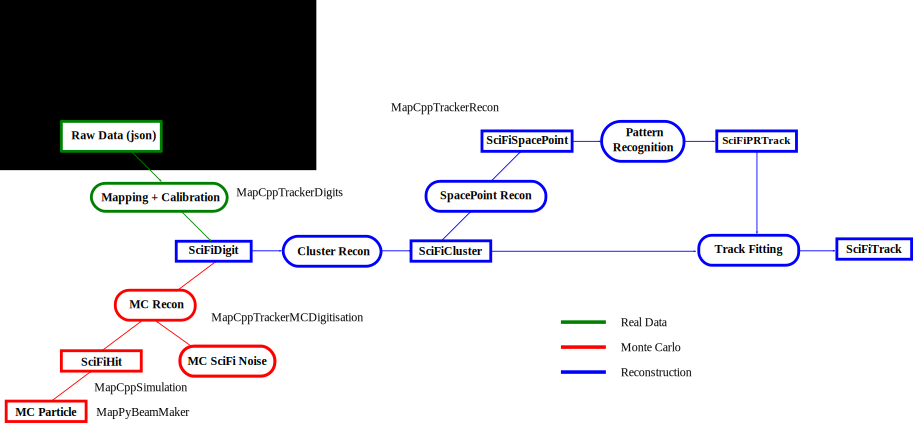
\includegraphics[width=0.95\linewidth]{07-Reconstruction/DataFlow2014.pdf}
    \caption{\label{fig:DataFlow} The reconstruction data flow. Data originates either from simulated or real data, the two branches meet after digitisation, after which the reconstruction proceeds identically for both.  The relevant MAUS modules for each step are indicated.}
  \end{center}
\end{figure}

  \subsection{Digitization}
  \label{subsec:Digitization}
  For real data the electronic signals produced by the VLPCs are digitised using analogue-to-digital converters (ADCs). The DAQ system records the pulse height for each DAQ channel.  Channel-by-channel cailbration constants are used to convert the ADC value to a signal in units of photo-electrons (PE) and the VLPC channel number to fibre number.  This information is then used to form a Digit.  The analagous process for Monte Carlo data is described in section~\ref{sec:Simulation}.

  \subsection{Clustering}
  \label{subsec:Clustering}
  A particle that traverses a plane will generate a hit in one or at most two adjacent channels.  An isolated hit or hits in two adjacent channels form a cluster.  
  
  The clustering algorithm loops over every combination of pairs of Digits in a SciFiEvent and combines any that occur in neighbouring channels in the same plane. The channel offset is then calculated by subtracting the central fibre channel number from the digit channel number. In the case of multi-digit cluster, the average channel value is used. From the channel offset the position in the  $(u,v,w)$ co-ordinate system can be detemined

  \subsection{Spacepoint Reconstruction}
  \label{subsec:SpacepointReconstruction}
  For each station the constituent planes are searched for clusters which can be used to define a Spacepoint. Spacepoints are defined by Clusters from all three planes (a triplet Spacepoint) or for any two out of the three planes (a doublet Spacepoint). 
  From the Cluster co-ordinates the $(x, y)$ coordinates of the Spacepoint are calculated.

  \subsubsection{Cluster selection}
  \label{subsubsec:ClusterSelection}
  In order to determine which Clusters from each plane originate from the same track we follow Kuno's conjecture\cite{MiceTrackers} which states that, for a given triplet Spacepoint, the sum of the channel numbers of each cluster will be a constant.  So if $n^u$, $n^v$ and $n^w$ are the fibre numbers of the Clusters in $u$, $v$ and $w$ and $n^u_0$, $n^v_0$ and $n^w_0$ are the corresponding central-fibre numbers. Three clusters form a space point  if:
  \begin{equation}
    | (n^u + n^v + n^w) - (n^u_0 + n^v_0 + n^w_0) | < K \, .
  \end{equation}
  where $K$ is a constant, take by default as 3.0.
  
  Once all triplet space-points have been found, doublet space-points are created from pairs of remaining Clusters. 

  % \subsubsection{Crossing Point Calculation}
  % \label{subsubsec:CrossingPointCalculation}

  \subsection{Pattern Recognition}
  \label{subsec:PatternRecognition}

  Pattern recognition is based on looping over different combinations of Spacepoints and performing a fit using a simple linear least squares technique.  The algorithm treats helical and straight tracks separately, though much of the code is shared. Helical track finding is attempted first then, once all possible helical tracks have been found, any remaining unmatched Spacepoints in the SciFiEvent are passed to the straight line fitting rountines.

   \subsubsection{Helical Pattern Recognition}
   \label{subsubsec:HelicalPatternRecognition}

   The helical pattern recognition is performed in cylindrical co-ordinates $(r, \phi, z)$ where the turning angle $\phi$ defined for $0 \rightarrow \infty$ is distinguished from $\phi '$ the reduced turing angle defined  for $0 \rightarrow 2\pi$. For the helix $s$ is the distance the particle travels measured along the helix. The helix is described by: the circle it describes in the transverse plane $(x_{centre}, y_{centre}, radius)$; $s_0$ the value of $s$ where the helix crosses the reference plane; and $t_s = ds/dz$, which describes the tightness of the coiling. $\phi_0$, the angle of the track as it crosses the tracker reference plane, equivalent to $s_0$, is also used. 

   To find a track one Spacepoint is selected from each station and a circle is fitted in the $(r, \phi')$ projection. If the $\chi^2$ of this fit is sufficiently small (by default less than 15.0 multiplied by the number of degrees of freedom) then the value of $\phi$ is used to generate $s$ and a straight line fit is performed in the $(z,s)$ plane, and if the $\chi^2$ in this projection is also small (by default less than 4.0 multiplied by the number of degrees of freedom) the track is accepted.  $\phi$ itself is determined from $\phi'$ by exploiting the different distances in $z$ between successive tracker stations.  The change in $\phi$ between the hits in any two stations, divided by the distance between those stations, gives a constant which is the same for any pair of hits.  This can then be used to infer the true values of $\phi$.

   All possible combinations of five Spacepoints, one from each station are tested. Points can only be associated with one track. Then all combinations of any remaining Spacepoints are searched, this time requiring Spacepoints from four out of the five stations to form a helix. Tracks with momentum almost parallel to the solenoid axis (i.e. with low transverse momentum, $p_T$) will not suffer an appreciable bend and will not be found by the helix search and so any Spacepoints remaining after the helical tracks have been found are passed to the straight track finding algorithm.

    \subsubsection{Straight Line Pattern Recognition}
    \label{subsubsec:StraightLinePatternRecognition}

    Straight lines are fitted to the Spacepoints when there is no magnetic field and on any Spacepoints remaining after the helix fit is complete. The latter is to identify tracks with a small $p_T$ which are not bent sufficiently in the magnetic field to form a recognisable helix (it has been observed from Monte Carlo studies that the efficiency of the helix finding algorithm begins to tail off for tracks with $p_T < 10 MeV/c$).

    The fit is done in Cartesian coordinates and the track parameters are: $(x_0, y_0, t_x, t_y)$ where $t_x = dx/dz$ and $t_y = dy/dz$. Two Spacepoints are chosen in the outer chambers and a road is created between them. Any Spacepoints in the road are fitted, using Least Sqaures, in the $(x,z)$ and $(y,z)$ planes. The Spacepoints with the lowest $\chi^2$ are chosen as long as their value is less than a predefined cut value (by default less than 15.0 multiplied by the number of degrees of freedom). As in the helical case, following the completion of the full 5 point track search, tracks with Spacepoints in 4 out of the 5 stations are searched for. For the straight case only, following the completetion of the search for 4 point tracks, a search is also made for tracks with Spacepoints in only 3 out of the 5 stations. 

   \subsection{Track Fit}
   \label{subsec:FinalTrackFit}
   The final track fit was implemented using a track-orientated Kalman filter\cite{Fruhwirth,Billoir}, which can be shown to be an optimal linear fitter that takes into account all correlations and measurements, under the assumption that the system and measurements have a linear response. For the helical track fit, the system is only approximately linear, hence an extended Kalman filter was implmented. This implementation analytically propagates the track states between measurements, while the associated covariance matrix is propagated using a linear approximation to the non-linear system.

   Pattern recognition provides a set of clusters that are associated with a track which passed the selection criteria, and a parameterisation of that track based on a least squares fit to the points by a helix or a straight line as appropriate. The track parameters calculated from the least squares fit are used to provide the seed for the Kalman fit and the raw cluster information is used as the measurement data. The flexibility of the Kalman algorithm permits the effects of individual planes (MCS and energy loss) to be accounted for between each measurement point.
   
   The track is modelled as function of $z$ (the direction of the beam) where each plane represents a trackpoint and contains a measurement and a track state. The ``process noise'', the statistical fluctuation in the track state between two planes, is modelled using approximations to multiple coulomb scattering and energy straggling. The ``measurement noise'', the statistical error associated with making a measurement of the track, corresponds the statistically error associated with making a measurement of the true track state. This was computed to be $w/\sqrt{12}$, which corresponds to the standard deviation of a top-hat function representing an individual channel width. Both the process noise and measurement noise are gaussian approximations to non-gaussian functions. Higher order approximations could be made in future to account for the non-linearity more rigorously.
   
   Starting from station~5, plane~2, in each tracker, the Kalman fit progresses towards station~1, plane~0, first predicting the state at the next plane before using the measurement information to improve on the prediction. This process is known as filtering and continues until all the planes have been included in the fit. Should a plane not contain a measurement, the predicted value is stored instead of the filtered value. Once the filtering stage is complete, the track is ``smoothed'' to ensure that the benefits of using all the measurement information is correctly distributed throughout the track. Smoothing involves propagting the track in reverse from station~1 to station~5 weighting the change in state by the effect of the subsequent measurements.

    \subsubsection{Goodness of fit}
    For each fitted track, a test statistic is computed, which is the $\chi^2$ sum over all the trackpoints. It is calculated by $\chi^2\sum_{k=0}^{k=n}\chi_k^2$ where each chisquared update is given by $\chi_{k}^{2}=\mathbf{r}_{k}^{T}\mathrm{R}_{k}^{-1}\mathbf{r}_{k}$: where $r_{k}$ is the residual computed from the filtered state vector. $r_{k}=\mathbf{m}_{k}-\mathrm{H}_{k}\mathbf{a}_{k}$: where $\mathbf{m}_{k}$ is the $k^{th}$  measured point; $\mathbf{a}_{k}$ is the best Kalman estimate of track state vector at the $k^{th}$ intersection point and $\mathrm{H}_{k}$ is the matrix which projects the state vector of the track into the measurement space. $\mathrm{R}_{k}$ is the covariance matrix of the residuals and is given by  $\mathrm{R}_{k}=\mathrm{V}_{k}-\mathrm{H}_{k}\mathrm{C}_{k}\mathrm{H}_{k}^{T}$ where $\mathrm{V}_{k}$ is the measurement covariance matrix and $\mathrm{C}_{k}$ is the projected variance matrix. This definition of  $\chi^{2}$  takes into account correlations in the measurement predictions and, combined with the number of degrees of freedom of the track fit, is used to generate a {\it p-value} for the track, which we use as a measure of fit quality.

    \subsubsection{Important Considerations}

%\begin{equation}
%\chi_{k}^{2}=\mathbf{r}_{k}^{T}\mathrm{R}_{k}^{-1}\mathbf{r}_{k}.
%\end{equation}





  

\section{Performance}
\label{sec:Performance}

  A high statistics Monte Carlo simulation was performed in order to estimate the reconstruction efficiency and resolution of the implemented track-finding and track-fitting algorithms. It was necessarily Monte Carlo based in order to compare the reconstructed events to the simulated truth, thereby highlighting any inefficiencies and inaccuracies within the algorithms, without any additional noise or biases.

  The fitted transverse positions, $(x,y)$, and momenta, $(p_x, p_y, p_z)$, were compared against the the Monte Carlo truth on an event-by-event basis. The reconstructed events were not subject to any cuts or additional requirements over those of real data reconstruction. The Monte Carlo truth data was determined from the simulated track information, which was stored at every tracker plane to permit a direct comparison to the reconstructed data. All data sets were compared at the tracker reference surface, the designated measurement location with the MICE cooling channel.

  An artificial beam was generated with uniform distributions in both the longintudinal and transverse momenta. This was to ensure that the results were not biased by the incoming beam distribution, and that the full reconstructable phase space was probed with equal statistics.

  \subsection{Track Finding Efficiency}
  \label{sec:performance:track_finding}

  For every simulated event, the number of expected tracks was calculated from the Monte Carlo truth. If the simulated track crossed enough tracker planes to create a sufficient number of spacepoints (3 for straight tracks and 4 for helical tracks), a reconstructed track was expected. The reconstructed tracks were then compared for each tracker and compared to the expected track parameters. The efficiency of track finding as a function of the true longtudinal and transverse momenta is shown in figure~\ref{fig:track_efficiency}.

  \begin{figure}[p]
    \centering
    \includegraphics[width=0.45\textwidth, angle=0]{08-Performance/upstream_pz_track_efficiency.pdf}
    \includegraphics[width=0.45\textwidth, angle=0]{08-Performance/downstream_pz_track_efficiency.pdf}\\
    \includegraphics[width=0.45\textwidth, angle=0]{08-Performance/upstream_pt_track_efficiency.pdf}
    \includegraphics[width=0.45\textwidth, angle=0]{08-Performance/downstream_pt_track_efficiency.pdf}
    \caption{\label{fig:track_efficiency} The efficiency of reconstructing tracks in the upstream (left) and downstream (right) trackers as a function of the simulated longitudinal (top) and transverse (bottom) momentum.}
  \end{figure}

  Once the the Monte Carlo tracks have been identified, the expected number of trackpoints can be calculated by examining the number of tracker planes that the simulated track crossed. Comparing the number of trackpoints in each reconstructed track to the expected number for each simulated track permits the efficiency of finding the correct number of trackpoints to be calculated. Figure~\ref{fig:tp_efficiency} shows the trackpoint finding efficiency as a function of longitudinal and transverse momenta.

  \begin{figure}[p]
    \centering
    \includegraphics[width=0.45\textwidth, angle=0]{08-Performance/upstream_pz_tp_efficiency.pdf}
    \includegraphics[width=0.45\textwidth, angle=0]{08-Performance/downstream_pz_tp_efficiency.pdf}\\
    \includegraphics[width=0.45\textwidth, angle=0]{08-Performance/upstream_pt_tp_efficiency.pdf}
    \includegraphics[width=0.45\textwidth, angle=0]{08-Performance/downstream_pt_tp_efficiency.pdf}
    \caption{\label{fig:tp_efficiency} The efficiency of reconstructing trackpoionts in the upstream (left) and downstream (right) trackers as a function of the simulated transverse momentum.}
  \end{figure}


  \subsection{Reconstruction Resolution}
  \label{sec:performance:resolutions}
  
  Position residuals are shown in figures~\ref{fig:XResidKalman} and \ref{fig:YResidKalman}, and the momentum residuals in figures~\ref{fig:PtResidKalman} and \ref{fig:PzResidKalman}.  The position reconstruction can be seen to agree with the Monte Carlo truth to high precision in both the upstream and downstream trackers. The momentum residuals currently display some systematic effect which is due to a known issue with the energy loss determination and is currently under study.
  
  In order to produce these plots, a requirement that there was a cluster within the reference plane was applied. Due to the effects of Multiple Coulomb Scattering, on rare occaisons a single hard scatter can cause pattern recognition to miss a single spacepoint at the reference plane, hence creating a tail that will adversely affect the distrubtions. As we are concerned with the resolution following a successful pattern recognition stage, these events were removed.
  
  The position residuals are consistent with the expected measurement resolutions for a combined fit and the absolute spread is very close to the width of a channel (1.497mm). The transverse momentum resolution is consitent accross the range of the sensitive phase space at $\sim$1~MeV/c in both trackers. The longitudinal momentum, an intrinsically more difficult measurement for the tracker, still retains an acceptable spread of $\sim2.7$~MeV/c in both trackers. There is however a systematic offset present in the distributions, $\sim0.8$~MeV/c in both trackers, and the distributions have more pronounced tails than in the transverse cases. These offsets require further investigation. It is believed that the root cause is a systematic under (over) estimation of the energy loss per plane in the upstream (downstream) tracker, which is realised in the 0.8~MeV/c longitudinal, and 0.2~MeV/c transverse, systematic offsets.
  
  Trends in transverse and longitudinal momentum resolution as a function of transverse momentum are shown in figures~\ref{fig:PtPtResolKalman} and \ref{fig:PtPzResolKalman}. A consistently uniform distribution is found in the transverse momentum as exected, with the predominant issue found in the longitudinal reconstruction of low-$P_t$ tracks. This effect, when coupled with variations in efficiency will yield some systematic concerns in the reconstruction of statistical quantities such as emittance. Studies of these systematic biases are currently underway.

  \begin{figure}[p]
    \begin{center}
      \includegraphics[width=0.49\textwidth, angle=0]{08-Performance/upstream_x_residual.pdf}
      \includegraphics[width=0.49\textwidth, angle=0]{08-Performance/downstream_x_residual.pdf}
      \caption{\label{fig:XResidKalman} The $x$ residuals of the upstream (left) and downstream (right) trackers for a 6~mm 4D emittance, and 200~MeV/c momentum beam.}
    \end{center}
  \end{figure}
  
    \begin{figure}[p]
    \begin{center}
      \includegraphics[width=0.49\textwidth, angle=0]{08-Performance/upstream_y_residual.pdf}
      \includegraphics[width=0.49\textwidth, angle=0]{08-Performance/downstream_y_residual.pdf}
      \caption{\label{fig:YResidKalman} The $y$ residuals of the upstream (left) and downstream (right) trackers for a 6~mm 4D emittance, and 200~MeV/c momentum beam.}
    \end{center}
  \end{figure}
  
  
  \begin{figure}[p]
    \begin{center}
      \includegraphics[width=0.49\textwidth, angle=0]{08-Performance/upstream_pt_residual.pdf}
      \includegraphics[width=0.49\textwidth, angle=0]{08-Performance/downstream_pt_residual.pdf}
      \caption{\label{fig:PtResidKalman} The $p_{\perp}$ residuals of the upstream (left) and downstream (right).}
    \end{center}
  \end{figure}
  
   \begin{figure}[p]
    \begin{center}
      \includegraphics[width=0.49\textwidth, angle=0]{08-Performance/upstream_pz_residual.pdf}
      \includegraphics[width=0.49\textwidth, angle=0]{08-Performance/downstream_pz_residual.pdf}
      \caption{\label{fig:PzResidKalman} The $p_z$ residuals of the upstream (left) and downstream (right) trackers for a 6~mm 4D emittance, and 200~MeV/c momentum beam.}
    \end{center}
  \end{figure}
  
  \begin{figure}[p]
   \begin{center}
     \includegraphics[width=0.49\textwidth, angle=0]{08-Performance/upstream_pt_resolution_pt.pdf}
     \includegraphics[width=0.49\textwidth, angle=0]{08-Performance/downstream_pt_resolution_pt.pdf}
     \caption{\label{fig:PtPtResolKalman} The $p_{\perp}$ resolution vs the $p_{\perp}$ of the upstream (left) and downstream (right).}
   \end{center}
  \end{figure}
  
  \begin{figure}[p]
   \begin{center}
     \includegraphics[width=0.49\textwidth, angle=0]{08-Performance/upstream_pz_resolution_pt.pdf}
     \includegraphics[width=0.49\textwidth, angle=0]{08-Performance/downstream_pz_resolution_pt.pdf}
     \caption{\label{fig:PtPzResolKalman} The $p_z$ resolution vs the $p_{\perp}$ of the upstream (left) and downstream (right).}
   \end{center}
  \end{figure}

\section{Conclusion}
\label{sec:Conclusion}
The performance of the final Kalman filter-based track fit has been evaluated by comparing Monte Carlo truth with reconstructed data, for the key tracker measurements of $x$, $y$, $p_{t}$ and $p_z$.  The observed performance in the transverse position and momentum measurements is excellent, for both the upstream and downstream trackers. The reconstruction resolution in $p_t$ and $p_z$ meet specification and will provide a sufficient degree of precision for the MICE physics program. 

The track model uses a simplification of the energy loss in the tracker planes which leads to the systematic shift discussed in section 8.3. Since the two trackers were constructed to be identical this shift will cancel in the calculation of energy loss. Monte Carlo studies will allow us to calculate a linear correction to the measured momentum and account for the small remaining shift. We will use measurements by other detectors in MICE to validate this correction.

If the approximations in the track model, and their effect on the track fits, limits the ability to measure cooling, the current Kalman filter can be upgraded to an adaptive Kalman filter where the energy loss is both modelled and estimated by the track fit. The fitter was written to accept such upgrades.

MICE will measure the transverse emittance of a muon beam which requires the determination of the beam covariance matrix. Our errors will be small and symmetric which will permit a simple covariance matrix correction to be applied and allow an accurate and reliable measurement of muon beam cooling. The tracker software is now used routinely in MICE data reconstruction, providing data for analysis and publication.

% There are, however, systematic effects present in the momentum reconstruction due to the complexity of modelling the density and thicknesses of the various materials within the tracker. The Monte Carlo model provides a more detailed description than could feasibly be implemented in the reconstruction, hence producing the residuals seen in section~\ref{sec:performance:resolutions}. This discrepancy will be representative of a physical systematic effect in the reconstruction of data and corresponds to the leading systematic effect in the tracker reconstruction.
% 
% Monte Carlo studies will be used to model the momentum discrepancy and provide a linear correction. The linear correction can then be used during analyses to reduce the effect of this systematic. Comparisons with other detectors in the MICE experiment may provide a data-driven estimate for this correction thereby supporting the Monte Carlo model. In addition it would be possible to further extend the track fit such that an Adaptive Kalman Filter is used, whereby the energy loss per plane is both modelled and estimated by the track fit. Such extensions are currently under discussion.
% 
% Due to the precision of the track fit the key measurement of MICE, the transverse emittance of a muon beam, meets specification. The emittance is based on the precise determination of the beam covariance matrix, and is therefore sensitive to the resolution of the reconstruction. The resolutions of the individual parameters are small and symmetric which permits a simple covariance matrix correction to be applied, fully accounting for the measurement effects of the tracker. Additionally, the high resolution reduces the number of muons required to acheive the expected statistical precision of MICE.

% The performance of the final Kalman filter-based track fit has been evaluated by comparing Monte Carlo truth with reconstructed data, for the key tracker measurements of $x$, $y$, $p_{t}$ and $p_z$.  The observed performance in the transverse position is excellent for both the upstream and downstream trackers. The reconstruction resolution in $p_t$ and $p_z$ meet specification and will provide a sufficient degree of precision for the MICE physics program.

%There are, however, systematic effects present in the momentum reconstruction due to the complexity of modelling the density and thicknesses of the various materials within the tracker. The Monte Carlo model provides a more detailed description than could feasibly be implemented in the reconstruction, hence producing the residuals seen in section~\ref{sec:performance:resolutions}. This discrepancy will be representative of a physical systematic effect in the reconstruction of data and corresponds to the leading systematic effect in the tracker reconstruction.

% Systematic effects are present in the momentum reconstruction, which have the potential to produce a corresponding systematic effect in the final emittance measurement unless accounted for. Monte Carlo studies will be used to model the momentum discrepancy and provide a linear correction. The linear correction can then be used during analyses to reduce the effect of this systematic. Comparisons with other detectors in the MICE experiment may provide a data-driven estimate for this correction thereby supporting the Monte Carlo model. In addition it would be possible to further extend the track fit such that an Adaptive Kalman Filter is used, whereby the energy loss per plane is both modelled and estimated by the track fit. Such extensions are currently under discussion.

%Due to the precision of the track fit the key measurement of MICE, the transverse emittance of a muon beam, meets specification. The emittance is based on the precise determination of the beam covariance matrix, and is therefore sensitive to the resolution of the reconstruction. The resolutions of the individual parameters are small and symmetric which permits a simple covariance matrix correction to be applied, fully accounting for the measurement effects of the tracker. Additionally, the high resolution reduces the number of muons required to acheive the expected statistical precision of MICE.


 \begin{figure}[p]
    \centering
    \includegraphics[width=0.85\textwidth, angle=0]{08-Performance/kuno_plot.pdf}
    \caption{\label{fig:kuno} A plot showing the sum of the channel numbers for the clusters in each spacepoint for the upstream (left) and downstream (right) trackers. Kuno's conjecture that the sum is a constant is observed with a small variation in the downstream tracker arising from a slight fibre misalignment during construction.}
  \end{figure}

  \begin{figure}[p]
    \centering
    \includegraphics[width=0.495\textwidth, angle=0]{08-Performance/upstream_track_efficiency.pdf}
    \includegraphics[width=0.495\textwidth, angle=0]{08-Performance/downstream_track_efficiency.pdf}\\
    \caption{\label{fig:track_efficiency} The efficiency of reconstructing tracks in the upstream (left) and downstream (right) trackers as a function of the simulated longitudinal and transverse momentum. The white area in the top left of the plot indicates events which fall outside of the $p_t/p_z$ ratio cut.}
  \end{figure}

%   \begin{figure}[p]
%     \centering
%     \includegraphics[width=0.45\textwidth, angle=0]{08-Performance/upstream_pz_track_efficiency.pdf}
%     \includegraphics[width=0.45\textwidth, angle=0]{08-Performance/downstream_pz_track_efficiency.pdf}\\
%     \includegraphics[width=0.45\textwidth, angle=0]{08-Performance/upstream_pt_track_efficiency.pdf}
%     \includegraphics[width=0.45\textwidth, angle=0]{08-Performance/downstream_pt_track_efficiency.pdf}
%     \caption{\label{fig:track_efficiency} The efficiency of reconstructing tracks in the upstream (left) and downstream (right) trackers as a function of the simulated longitudinal (top) and transverse (bottom) momentum.}
%   \end{figure}
  
%   \begin{figure}[p]
%     \centering
%     \includegraphics[width=0.45\textwidth, angle=0]{08-Performance/upstream_pz_tp_efficiency.pdf}
%     \includegraphics[width=0.45\textwidth, angle=0]{08-Performance/downstream_pz_tp_efficiency.pdf}\\
%     \includegraphics[width=0.45\textwidth, angle=0]{08-Performance/upstream_pt_tp_efficiency.pdf}
%     \includegraphics[width=0.45\textwidth, angle=0]{08-Performance/downstream_pt_tp_efficiency.pdf}
%     \caption{\label{fig:tp_efficiency} The efficiency of reconstructing trackpoints in the upstream (left) and downstream (right) trackers as a function of the simulated longitudinal (top) and transverse (bottom) momentum.}
%   \end{figure}
  
  \begin{figure}[p]
   \centering
    \includegraphics[width=0.49\textwidth, angle=0]{08-Performance/chi_squared_ndf_up.pdf}
    \includegraphics[width=0.49\textwidth, angle=0]{08-Performance/chi_squared_ndf_down.pdf}
   \caption{\label{fig:track_chisq} The $\chi^2$ per degree of freedom in the upstream (left) and downstream (right) trackers.}
  \end{figure}
  
  \begin{figure}[p]
    \begin{center}
      \includegraphics[width=0.49\textwidth, angle=0]{08-Performance/upstream_x_residual.pdf}
      \includegraphics[width=0.49\textwidth, angle=0]{08-Performance/downstream_x_residual.pdf}
      \caption{\label{fig:XResidKalman} The $x$ residuals of the upstream (left) and downstream (right) trackers.}
    \end{center}
  \end{figure}
  
    \begin{figure}[p]
    \begin{center}
      \includegraphics[width=0.49\textwidth, angle=0]{08-Performance/upstream_y_residual.pdf}
      \includegraphics[width=0.49\textwidth, angle=0]{08-Performance/downstream_y_residual.pdf}
      \caption{\label{fig:YResidKalman} The $y$ residuals of the upstream (left) and downstream (right) trackers.}
    \end{center}
  \end{figure} 
  
  \begin{figure}[p]
    \begin{center}
      \includegraphics[width=0.49\textwidth, angle=0]{08-Performance/upstream_pt_residual.pdf}
      \includegraphics[width=0.49\textwidth, angle=0]{08-Performance/downstream_pt_residual.pdf}
      \caption{\label{fig:PtResidKalman} The $p_{t}$ residuals of the upstream (left) and downstream (right) trackers.}
    \end{center}
  \end{figure}
  
   \begin{figure}[p]
    \begin{center}
      \includegraphics[width=0.49\textwidth, angle=0]{08-Performance/upstream_pz_residual.pdf}
      \includegraphics[width=0.49\textwidth, angle=0]{08-Performance/downstream_pz_residual.pdf}
      \caption{\label{fig:PzResidKalman} The $p_z$ residuals of the upstream (left) and downstream (right) trackers.}
    \end{center}
  \end{figure}
  
%   \begin{figure}[p]
%     \begin{center}
%       \includegraphics[width=0.49\textwidth, angle=0]{08-Performance/upstream_p_bias_p.pdf}
%       \includegraphics[width=0.49\textwidth, angle=0]{08-Performance/downstream_p_bias_p.pdf}
%       \caption{\label{fig:pBiasKalman} The mean residual between the final track fit total momentum and the true track momentum, evaluated at the reference plane.}
%     \end{center}
%   \end{figure}
  
  \begin{figure}[p]
   \begin{center}
     \includegraphics[width=0.49\textwidth, angle=0]{08-Performance/upstream_pt_resolution_pt.pdf}
     \includegraphics[width=0.49\textwidth, angle=0]{08-Performance/downstream_pt_resolution_pt.pdf}
     \caption{\label{fig:PtPtResolKalman} The $p_{t}$ resolution as a function of the $p_{t}$ of the upstream (left) and downstream (right) trackers.}
   \end{center}
  \end{figure}
  
  \begin{figure}[p]
   \begin{center}
     \includegraphics[width=0.49\textwidth, angle=0]{08-Performance/upstream_pz_resolution_pt.pdf}
     \includegraphics[width=0.49\textwidth, angle=0]{08-Performance/downstream_pz_resolution_pt.pdf}
     \caption{\label{fig:PtPzResolKalman} The $p_z$ resolution vs the $p_{t}$ of the upstream (left) and downstream (right) trackers.}
   \end{center}
  \end{figure}


\clearpage

\bibliography{MICE_2014-05}                                                                           
\bibliographystyle{99-Styles/utphys}


% \cleardoublepage
% \appendix
% \input 11-AuthorList/11-AuthorList

\end{document}
